\pgfplotsset{compat=1.17}     
        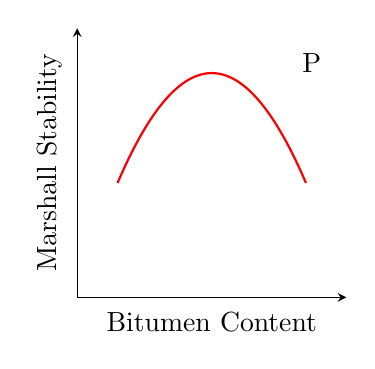
\begin{tikzpicture}
            \begin{axis}[
                xlabel={Bitumen Content},
                ylabel={Marshall Stability},
                xmin=0, xmax=1,
                ymin=0, ymax=1.2,
                axis lines=left,
                width=5cm, height=5cm,
                xtick=\empty, ytick=\empty,
            ]
                \addplot[domain=0.15:0.85, samples=100, thick, red] {4*x*(1-x)};
                \node[anchor=south west] at (rel axis cs:0.8,0.8) {P};
            \end{axis}
        \end{tikzpicture}
    \hfill
        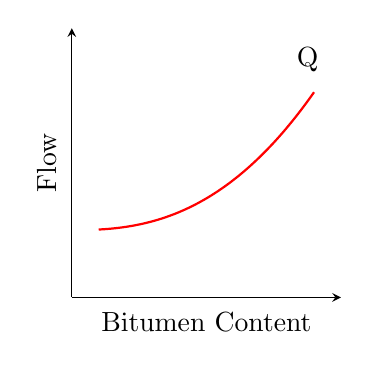
\begin{tikzpicture}
            \begin{axis}[
                xlabel={Bitumen Content},
                ylabel={Flow},
                xmin=0, xmax=1,
                ymin=0, ymax=1.2,
                axis lines=left,
                width=5cm, height=5cm,
                xtick=\empty, ytick=\empty,
            ]
                \addplot[domain=0.1:0.9, samples=100, thick, red] {0.3 + 0.8*x^2.5};
                \node[anchor=south west] at (rel axis cs:0.8,0.8) {Q};
            \end{axis}
        \end{tikzpicture}
    \vskip\baselineskip 
        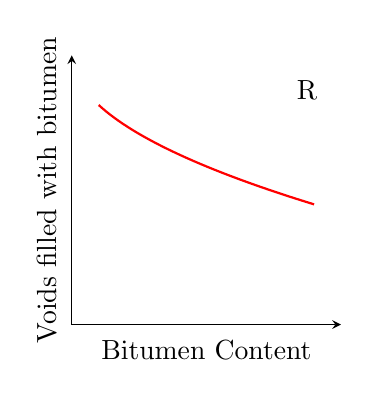
\begin{tikzpicture}
            \begin{axis}[
                xlabel={Bitumen Content},
                ylabel={Voids filled with bitumen},
                xmin=0, xmax=1,
                ymin=0, ymax=1.2,
                axis lines=left,
                width=5cm, height=5cm,
                xtick=\empty, ytick=\empty,
            ]
                \addplot[domain=0.1:0.9, samples=100, thick, red] {1.2 - 0.7*x^0.5};
                \node[anchor=south west] at (rel axis cs:0.8,0.8) {R};
            \end{axis}
        \end{tikzpicture}
    \hfill
        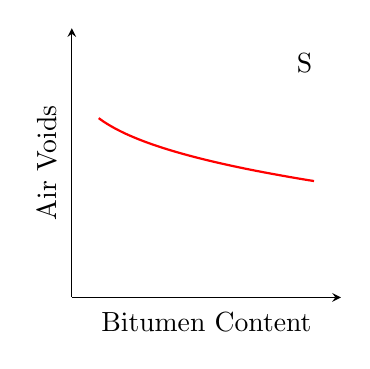
\begin{tikzpicture}
            \begin{axis}[
                xlabel={Bitumen Content},
                ylabel={Air Voids},
                xmin=0, xmax=1,
                ymin=0, ymax=1.2,
                axis lines=left,
                width=5cm, height=5cm,
                xtick=\empty, ytick=\empty,
            ]
                \addplot[domain=0.1:0.9, samples=100, thick, red] {1.1 - 0.6*x^0.3};
                \node[anchor=south west] at (rel axis cs:0.8,0.8) {S};
            \end{axis}
        \end{tikzpicture}
